\section{语法分析程序}
项目复用了前一次语法分析实验的内容,在LexicalAnalysis\footnote{https://github.com/shellqiqi/LexicalAnalysis} 中描述了词法分析的细节,本节不介绍相关的代码细节。
\subsection{程序结构}
本程序分两个包,\verb|lexer|包包含词法分析类,\verb|parser|包包含语法分析类,\verb|App|作为入口类。\verb|lexer|中有三个类,\verb|DFA|类从~\verb|resource|中读取一个状态转化表,\verb|Lexer|类做词法分析,\verb|Token|是一个词素。\verb|parser|中有四个类,\verb|Parser|类做语法分析并给出语法分析树,\verb|SyntaxTree|类由~\verb|SyntaxTreeNode|类与~\verb|TokenNode|类组合而来,表示一个语法分析树。资源文件包括一个由Mini-C编写的程序以及识别语言的状态转化表。
\subsection{语法分析树数据结构}
\begin{figure}[htbp]
    \centering
    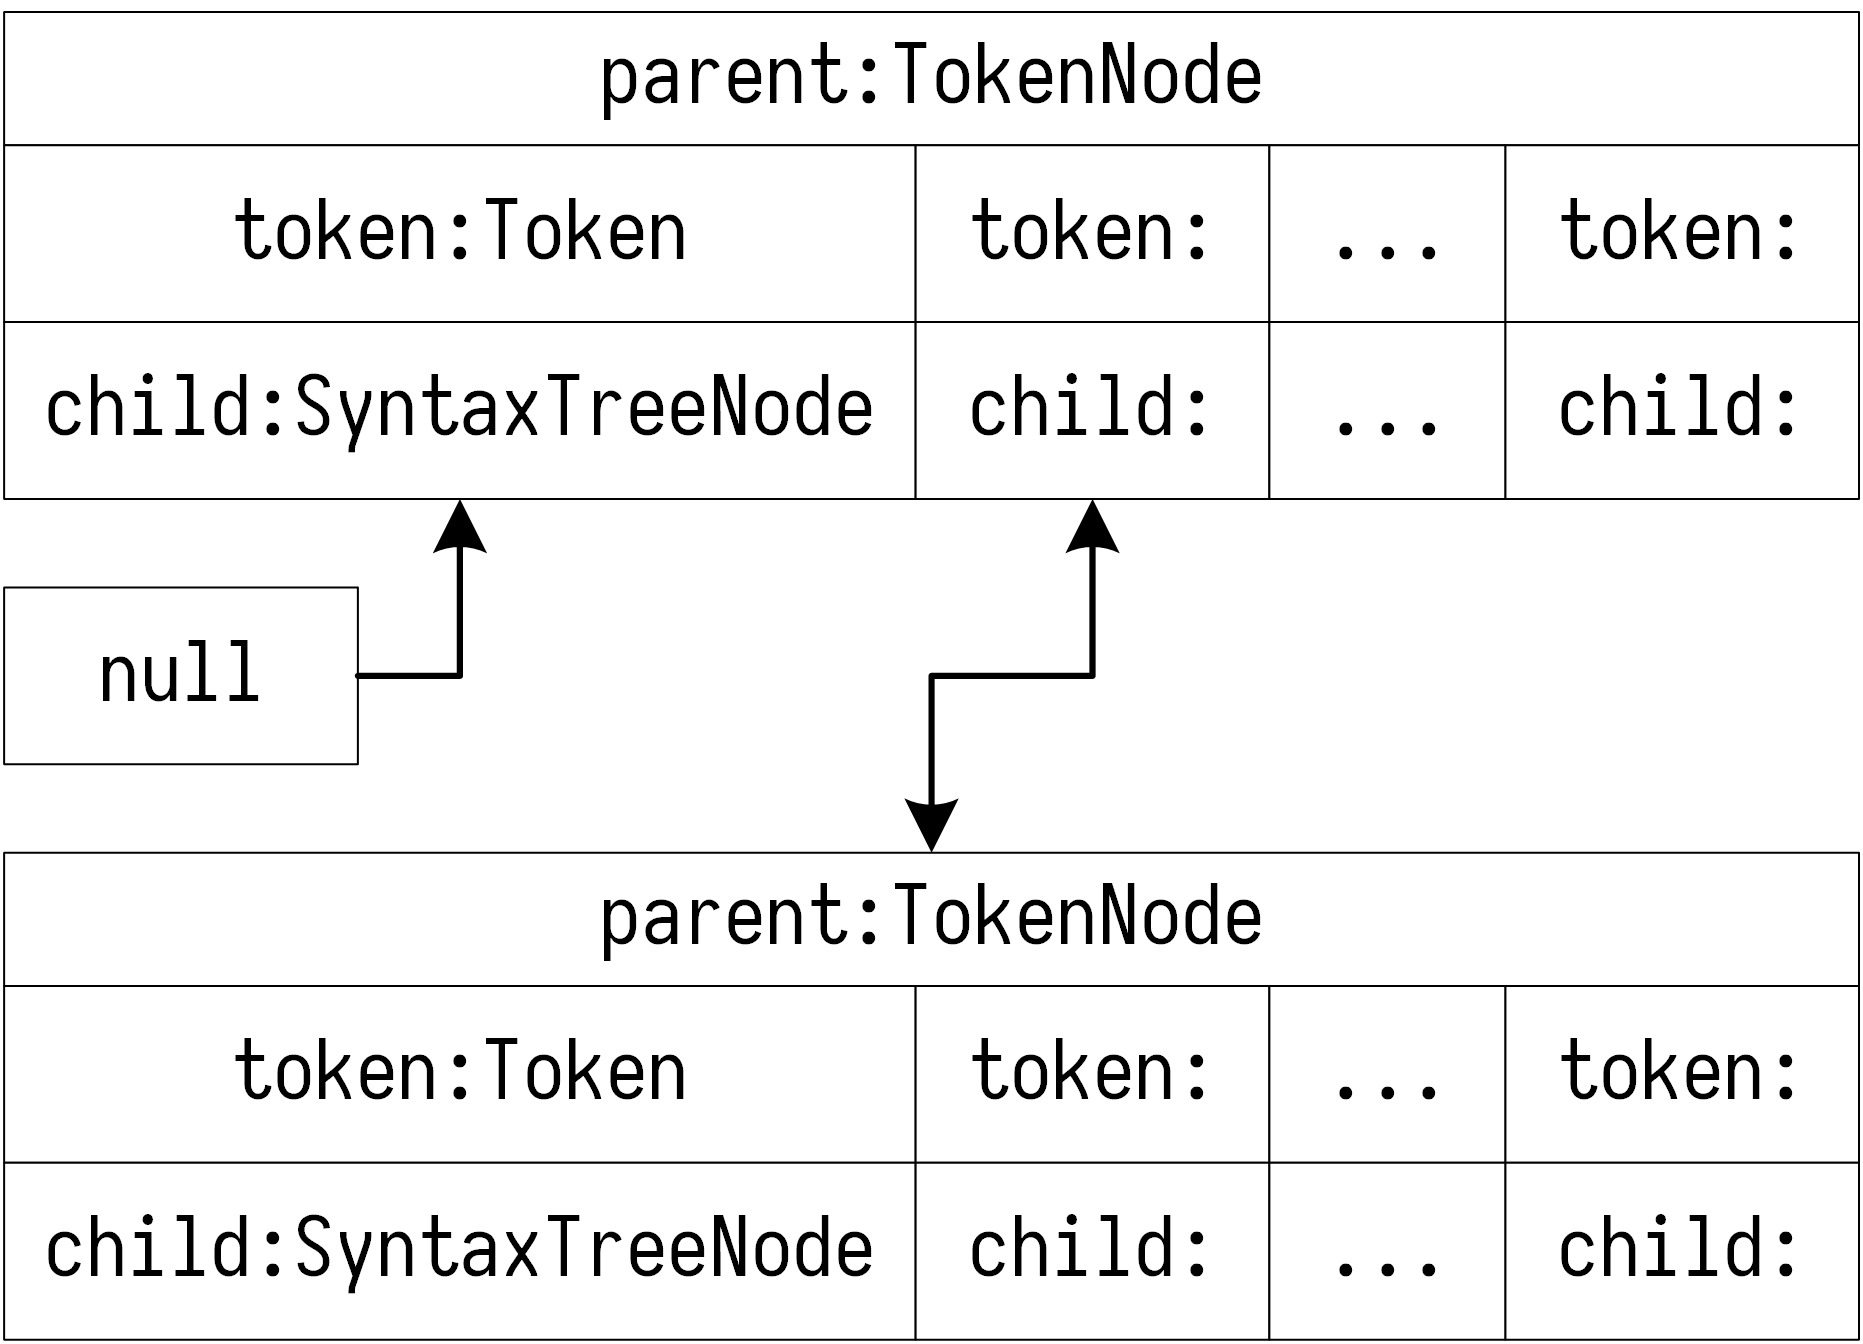
\includegraphics{../assets/SyntaxTree.png}
    \caption{语法分析树数据结构}
\end{figure}
\subsection{程序源码}
\subsubsection{\texttt{Parser}类程序清单}
{\linespread{1}
\lstinputlisting[caption=Parser.java]{../src/main/java/shell7/parser/Parser.java}}
\subsubsection{\texttt{SyntaxTree}类程序清单}
语法分析树类保存了树的根节点和根上~\verb|Token|列表的栈操作。
{\linespread{1}
\lstinputlisting[caption=SyntaxTree.java]{../src/main/java/shell7/parser/SyntaxTree.java}}
\subsubsection{\texttt{SyntaxTreeNode}类程序清单}
语法分析树结点保持了该结点的亲属和一个~\verb|Token|列表。
{\linespread{1}
\lstinputlisting[caption=SyntaxTreeNode.java]{../src/main/java/shell7/parser/SyntaxTreeNode.java}}
\subsubsection{\texttt{TokenNode}类程序清单}
\verb|Token|结点保持了一个终结符或一个非终结符的一个展开。
{\linespread{1}
\lstinputlisting[caption=TokenNode.java]{../src/main/java/shell7/parser/TokenNode.java}}
\subsection{测试结果}
{\linespread{1}
\begin{lstlisting}[caption=测试结果]
S
S -> IF B S ELSE S
    B -> ( ID )
    S -> IF B S ELSE S
        B -> ( ID )
        S -> ID ;
        S -> ID ;
    S -> IF B S
        B -> ( ID )
        S -> ID ;
\end{lstlisting}}